\documentclass[a4paper]{article}
\usepackage[14pt]{extsizes}
\usepackage[T2A]{fontenc}
\usepackage[top=15mm, bottom=20mm, left=25mm, right=20mm]{geometry}
\usepackage[russian]{babel}
\usepackage{tocloft}
\usepackage{graphicx}
\usepackage{float}
\usepackage{listings}
\usepackage{xcolor} % для цветовой подсветки
\usepackage{url}

\usepackage[linesnumbered,boxed]{algorithm2e}

\lstset{
	% Основные параметры
	basicstyle=\ttfamily\small,          % Моноширинный шрифт небольшого размера
	backgroundcolor=\color{white},       % Цвет фона
	showspaces=false,                    % Показывать ли пробелы
	showstringspaces=false,              % Показывать ли пробелы в строках
	showtabs=false,                      % Показывать ли табуляцию
	tabsize=4,                          % Размер табуляции (4 пробела)
	frame=single,                       % Рамка вокруг кода
	framerule=0.8pt,                    % Толщина рамки
	rulecolor=\color{gray!30},          % Цвет рамки
	captionpos=b,
	% Нумерация строк
	numbers=left,                       % Нумерация слева
	numberstyle=\tiny\color{gray},      % Стиль номеров строк
	numbersep=5pt,                      % Отступ номеров от кода
	stepnumber=1,                       % Шаг нумерации
	% Переносы
	breaklines=true,                    % Автоматический перенос строк
	breakatwhitespace=true,             % Перенос только по пробелам
	% Подсветка синтаксиса
	commentstyle=\color{green!50!black},% Стиль комментариев
	keywordstyle=\color{blue},          % Стиль ключевых слов
	stringstyle=\color{red},            % Стиль строк
	identifierstyle=\color{black},      % Стиль идентификаторов
}


\begin{document}
\begin{center}
	\thispagestyle{empty}
	\linespread{1.3}
	\MakeUppercase{министерство науки и высшего образования российской федерации}
	
	\normalsize
	федеральное государственное автономное образовательное учреждение высшего образования "<Санкт-Петербургский политехнический университет Петра Великого">
	
	\vspace{0.3cm}Институт компьютерных наук и кибербезопасности
	
	\vspace{0.3cm}Высшая школа технологий искусственного интеллекта
	
	\vspace{0.3cm}Направление: 02.03.01 Математика и компьютерные науки
	
	\vspace{2cm}\large
	КУРСОВАЯ РАБОТА
	
	ПО ДИСЦИПЛИНЕ АЛГОРИТМИЗАЦИЯ И ПРОГРАММИРОВАНИЕ
	
	на тему: "Разработка алгоритма принятия решений для игры в «Крестики-нолики» для пяти в ряд”
	
	\vspace{4cm}
\end{center}

\normalsize
Отчет выполнил

студент группы №5130201/40001 \hfill  \rule{2.7cm}{0.01cm} Шемякина Е. К.

\vspace{1cm}
Отчет принял

преподаватель \hfill  \rule{2.7cm}{0.01cm}  \hspace{0.25cm} Сеннов В. Н.

\vspace{1cm}
\begin{flushright}
	"<\rule{1cm}{0.01cm}"> \rule{3cm}{0.01cm}2025 г.
\end{flushright}

\begin{center}
	\small
	\vspace{2cm}Санкт-Петербург, 2025
\end{center}
\clearpage

\normalsize
\renewcommand{\cftsecleader}{\cftdotfill{\cftdotsep}}
\renewcommand{\cftdotsep}{1}
\tableofcontents
\clearpage


\section*{Введение}
\addcontentsline{toc}{section}{Введение}

Крестики-нолики — одна из самых известных и популярных настольных игр, которая сочетает в себе простоту правил и глубину стратегического мышления. Несмотря на кажущуюся элементарность, игра представляет значительный интерес с точки зрения алгоритмизации и искусственного интеллекта, особенно в модификациях с увеличенным полем и количеством символов для победы. Разработка алгоритмов, способных эффективно играть в такие вариации игры, является актуальной задачей, находящей применение в области теории игр, машинного обучения и разработки интеллектуальных систем.

Целью данной курсовой работы является разработка и реализация алгоритма для бота, способного играть в крестики-нолики на поле размером от 15×15 и более с условием победы при составлении линии из пяти или более символов. Алгоритм должен быть не только эффективным с точки зрения времени принятия решений, но и достаточно сильным, чтобы побеждать базового игрока, предоставленного в рамках проекта.

Работа представляет интерес для студентов, изучающих программирование и алгоритмы, так как позволяет применить теоретические знания на практике, развить навыки проектирования и оптимизации программных решений. Кроме того, результаты работы могут быть использованы в образовательных целях, для проведения турниров между алгоритмами, а также как основа для более сложных систем искусственного интеллекта.
\clearpage

\section{Постановка задачи}

В рамках курсовой работы требуется разработать и реализовать алгоритм для бота, играющего в крестики-нолики на поле размером MxN (M, N $\geq$ 15) с условием победы при построении линии из L = 5 одинаковых символов по горизонтали, вертикали или диагонали.

Исходные данные и условия:
\begin{enumerate}
	\item Предоставлен каркас проекта на C++17, включающий:
	\begin{itemize}
		\item Реализацию логики игры (библиотека tttcore), классы State и Game для управления состоянием и процессом игры.
		\item Интерфейс IPlayer, который должен быть реализован разрабатываемым алгоритмом.
		\item Интерфейс IObserver для получения событий из игры.
		\item Исполняемые модули для тестирования (tests) и игры по сети (tttremote).
		\item Закрытую библиотеку (libtttcore.a) с реализацией базового игрока ("baseline player") разумного, но не оптимального уровня, который будет использоваться как основной оппонент для тестирования.
		 
	\end{itemize}
	\item Алгоритм должен быть реализован в виде класса-наследника IPlayer и интегрирован в проект. Класс должен корректно работать с предоставленным API:
	\begin{itemize}
		\item Получать свой знак (X или O) через метод set\_sign.
		\item Принимать текущее состояние игры (const State \&) в методе make\_move.
		\item Возвращать координаты (row, col) следующего хода, которые должны находиться в пределах игрового поля и указывать на свободную клетку.
	\end{itemize}
	\item К алгоритму предъявляются следующие требования:
	\begin{itemize}
		\item Эффективность: Время вычисления одного хода не должно превышать 50 мс на стандартной рабочей станции.
		\item Сила игры: Разработанный бот должен стабильно обыгрывать предоставленного базового игрока (baseline player) в большинстве партий (за обе стороны — и за крестики, и за нолики).
		\item Универсальность: Алгоритм должен быть применим для полей разного размера (начиная от 15x15) и корректно обрабатывать все правила игры, включая предоставление последнего хода ноликам в случае потенциальной победы крестиков.
		
	\end{itemize}
	\item Критерии успешности выполнения работы:
	\begin{itemize}
		\item Алгоритм реализован, интегрирован в проект и проходит все предусмотренные тесты.
		\item Реализация побеждает базового бота в более чем 50\% случаев в сериях игр (например, 100 партий за крестики и 100 за нолики).
		\item Время принятия решений укладывается в заданные ограничения.
		\item Составлен подробный отчет, описывающий алгоритм, его реализацию и результаты тестирования.
		 
	\end{itemize}
\end{enumerate}
\clearpage

\section{Математическое описание}
\subsection{Модель игры}
Игровое поле представляет собой матрицу размера MxN (M, N $\geq$ 15). Каждая клетка может находиться в одном из трех состояний: пустая, занятая крестиком (X) или ноликом (O).
Выигрышное состояние - непрерывная последовательность из L=5 одинаковых символов по горизонтали, вертикали или диагонали.

\subsection{Описание алгоритма}
Алгоритм представляет собой систему правил, которые последовательно применяются к текущему состоянию поля для выбора наилучшей клетки для хода. Правила расположены в порядке убывания приоритета: как только находится ход, удовлетворяющий правилу, последующие правила не проверяются.

\textbf{Правило 1: Немедленная победа.}

\begin{itemize}
	\item Цель: Закончить игру своим выигрышем.
	\item Действие: Просканировать все пустые клетки на поле. Для каждой пустой клетки мысленно поставить в нее свой символ. Проверить, образует ли эта установка символа где-либо на поле линию длиной 5 или более своих символов. Если такая клетка найдена, выбрать ее для хода.
\end{itemize}

\textbf{Правило 2: Немедленная блокировка.}

\begin{itemize}
	\item Цель: Не позволить противнику выиграть на следующем ходу.
	\item Действие: Просканировать все пустые клетки на поле. Для каждой пустой клетки мысленно поставить в нее символ противника. Проверить, образует ли эта установка символа противника где-либо на поле линию длиной 5 или более его символов. Если такая клетка найдена, выбрать ее для хода (чтобы заблокировать победу противника).
	
\end{itemize}

\textbf{Правило 3: Создание двойной угрозы.}

\begin{itemize}
	\item Цель: Создать ситуацию, при которой противник не сможет предотвратить поражение на следующий ход, так как ему придется блокировать две угрозы одновременно.
	\item Действие: Просканировать все пустые клетки на поле. Для каждой пустой клетки мысленно поставить в нее свой символ. Далее, необходимо оценить, создает ли этот ход две или более отдельные угрозы.
	
	\item Определение угрозы: Угроза — это такая конфигурация символов на поле, при которой на следующем ходу игрок гарантированно может завершить линию из 5 символов. Простейший пример — незаблокированная последовательность из четырех своих символов, где с одной или двух сторон есть свободные клетки для пятого.
	
	\item Вывод: Если находится клетка, установка в которую своего символа создает две или более независимые угрозы, выбрать эту клетку для хода. Противник, способный блокировать только одну угрозу за ход, проиграет.
	
\end{itemize}



\textbf{Правило 4: Блокировка сильной атаки противника.}

\begin{itemize}
	\item Цель: Заблокировать потенциально выигрышную последовательность противника до того, как она превратится в немедленную угрозу (как в Правиле 2).
	
	\item Действие: Искать на поле конфигурации символов противника, которые являются "опасными". Например, не заблокированная последовательность из трех его символов, с обеих сторон от которой есть свободные клетки. Установка своего символа в одну из ключевых клеток, мешающих развитию этой последовательности, считается сильным блокирующим ходом.
	
\end{itemize}


\textbf{Правило 5: Развитие собственной атаки.}

\begin{itemize}
	\item Цель: Усилить свои позиции, создавая новые или продлевая существующие перспективные последовательности.
	
	\item Действие: Найти на поле все свои самые длинные незаблокированные последовательности (например, из 2 или 3 символов). Для каждой такой последовательности определить пустые клетки на ее продолжении. Выбрать ход в одну из этих клеток, отдавая предпочтение тем, которые продлевают самые длинные последовательности или находятся в центре.
	
\end{itemize}

\textbf{Правило 6: Стратегический выбор.}

\begin{itemize}
	\item Цель: Захватить наиболее выгодные позиции в начале игры или при отсутствии явных тактических вариантов.
	
	\item Действие: Если предыдущие правила не сработали (например, в самом начале игры), выбирать клетки согласно заранее заданному приоритету. Наивысший приоритет имеют клетки, расположенные ближе к центру поля, так как они предоставляют максимальное количество возможностей для построения линий во всех направлениях. Используется концепция "колец" вокруг центральной точки поля.
	
\end{itemize}

\textbf{Правило 7: Случайный выбор.}

\begin{itemize}
	\item Цель: Сделать корректный ход в ситуации, когда все вышеперечисленные стратегические и тактические соображения неприменимы (крайне редкий случай).
	
	\item Действие: Выбрать любую свободную клетку на поле случайным образом. Это гарантирует, что алгоритм всегда сможет сделать ход.
	
\end{itemize}

\clearpage

\section{Особенности реализации}

\begin{enumerate}
	\item Структуры данных и внутреннее представление состояния
	
	Для эффективного анализа игровой ситуации реализовано внутреннее представление игрового поля в виде двумерного массива m\_board типа Sign**. Размеры поля хранятся в переменных m\_rows и m\_cols. Данная структура была выбрана для обеспечения быстрого произвольного доступа к клеткам поля в процессе анализа.
	
	Инициализация и обновление доски происходит в методах:
	\begin{itemize}
		\item initialize\_board(const State\& state) - выделяет память и инициализирует массив значениями Sign::NONE.
		
		\item update\_board(const State\& state) - синхронизирует внутреннее представление с текущим состоянием игры.
	\end{itemize}
	
	\item Реализация алгоритма принятия решений
	
	Основная логика алгоритма реализована в методе make\_move(const State \&state), который последовательно применяет правила выбора хода в порядке убывания приоритета.  Функция приведена в листинге 1.
	
	\begin{lstlisting}[language=C++, caption={Функция выбора хода}]
		Point MyPlayer::make_move( const State &state )
		{
			Point result;
			
			if (state.get_move_no() == 0)
			{
				result.x = state.get_opts().cols / 2;
				result.y = state.get_opts().rows / 2;
				return result;
			}
			
			update_board(state);
			
			Sign enemy_sign = (m_sign == Sign::X) ? Sign::O : Sign::X;
			
			if (find_win_move(result, m_sign)) return result;           
			if (find_block_move(result, enemy_sign, 4)) return result;  
			if (find_double_threat(result, m_sign)) return result;      
			if (find_block_move(result, enemy_sign, 3)) return result;  
			if (find_strategic_move(result, m_sign)) return result;     
			
			for (int attempt = 0; attempt < 50; attempt++)
			{
				result.x = std::rand() % m_cols;
				result.y = std::rand() % m_rows;
				
				if (m_board[result.y][result.x] == Sign::NONE)
				{
					for (int dy = -1; dy <= 1; dy++)
					{
						for (int dx = -1; dx <= 1; dx++)
						{
							if (dx == 0 && dy == 0)
							continue;
							int nx = result.x + dx;
							int ny = result.y + dy;
							if (nx >= 0 && nx < m_cols && ny >= 0 && ny < m_rows && m_board[ny][nx] != Sign::NONE)
							return result;
						}
					}
				}
			}
			
			if (find_any_move(result))
			return result;
			
			result.x = 0;
			result.y = 0;
			return result;
		}
	\end{lstlisting}
	\item Ключевые вспомогательные методы
	Анализ линий: Метод check\_line(int x, int y, int dx, int dy, Sign sign) проверяет потенциальную линию в двух направлениях от заданной точки. Код функции представлен в листинге 2.
	
	\begin{lstlisting}[language=C++, caption={Функция анализа линий}]
		int MyPlayer::check_line( int x, int y, int dx, int dy, Sign sign ) const
		{
			int count = 0;
			int max_count = 0;
			
			for (int dir = -1; dir <= 1; dir += 2)
			{
				count = 0;
				for (int i = 1; i <= 4; i++)
				{
					int nx = x + i * dx * dir;
					int ny = y + i * dy * dir;
					
					if (nx < 0 || nx >= m_cols || ny < 0 || ny >= m_rows) break;
					if (m_board[ny][nx] == sign) count++;
					else if (m_board[ny][nx] == Sign::NONE) break;
					else { count = 0; break; }
				}
				max_count += count;
			}
			return max_count;
		}
	\end{lstlisting}
	
	Поиск выигрышного хода: find\_win\_move ищет ход, завершающий линию из 5 символов. Код функции представлен в листинге 3.
	
	\begin{lstlisting}[language=C++, caption={Функция поиска выигрышного кода}]
		bool MyPlayer::find_win_move( Point &result, Sign sign ) const
		{
			for (int y = 0; y < m_rows; y++)
			{
				for (int x = 0; x < m_cols; x++)
				{
					if (m_board[y][x] != Sign::NONE) continue;
					
					int directions[4][2] = {{1, 0}, {0, 1}, {1, 1}, {1, -1}};
					
					for (int d = 0; d < 4; d++)
					{
						if (check_line(x, y, directions[d][0], directions[d][1], sign) >= 4)
						{
							result.x = x; result.y = y;
							return true;
						}
					}
				}
			}
			return false;
		}
	\end{lstlisting}
	
	Поиск двойной угрозы: find\_double\_threat реализует ключевую идею алгоритма. Код функции представлен в листинге 4.
	
	\begin{lstlisting}[language=C++, caption={Функция поиска двойной угрозы}]
		bool MyPlayer::find_double_threat(Point& result, Sign sign) const
		{
			for (int y = 0; y < m_rows; y++)
			{
				for (int x = 0; x < m_cols; x++)
				{
					if (m_board[y][x] != Sign::NONE) continue;
					
					int threat_count = 0;
					int directions[4][2] = {{1, 0}, {0, 1}, {1, 1}, {1, -1}};
					
					for (int d = 0; d < 4; d++)
					{
						if (check_line(x, y, directions[d][0], directions[d][1], sign) >= 2)
						{
							threat_count++;
							if (threat_count >= 2)
							{
								result.x = x; result.y = y;
								return true;
							}
						}
					}
				}
			}
			return false;
		}
	\end{lstlisting}
	
	\item Генерация случайных чисел
	
	Для случайного выбора хода используется стандартная функция std::rand(). В цикле осуществляется до 50 попыток найти подходящую случайную клетку, предпочтительно рядом с уже занятыми клетками.
	
	\item Программный интерфейс
	
	Класс MyPlayer наследует интерфейс IPlayer и реализует:
	
	\begin{itemize}
		\item set\_sign(Sign sign) - установка знака игрока.
		\item make\_move(const State \&game) - основной метод выбора хода.
		\item get\_name() const - возврат имени игрока.
	\end{itemize}
	Приватные методы обеспечивают модульность реализации различных аспектов алгоритма, что упрощает тестирование и модификацию.
	
	\item Оптимизации
	
	Для обеспечения производительности реализованы:
	
	\begin{itemize}
		\item локальное кэширование состояния поля,
		\item поиск только в релевантных направлениях (4 основных направления),
		\item ранний выход из циклов при нахождении подходящего хода,
		\item ограничение количества проверяемых случайных клеток (50 попыток).
	\end{itemize}
	
\end{enumerate} 
\clearpage

\section{Результаты работы программы}

Для всесторонней оценки эффективности разработанного алгоритма были проведены серии тестовых партий, состоящие из 1000 игр, в различных конфигурациях. Тестирование проводилось на одном и том же устройстве с процессором Intel Core i5-11400H.

\begin{enumerate}
	\item Тестирование против простого игрока
	Простой игрок выбирает клетку для хода случайным образом, поэтому бот обыгрывает игрока в 100\% случаев.
	
	\item Тестирование против базового игрока
	
	Было проведено две серии тестов по 1000 игр. На рис. 1 и 2 представлены результаты тестов.
	
	\begin{figure}[H]
		\centering
		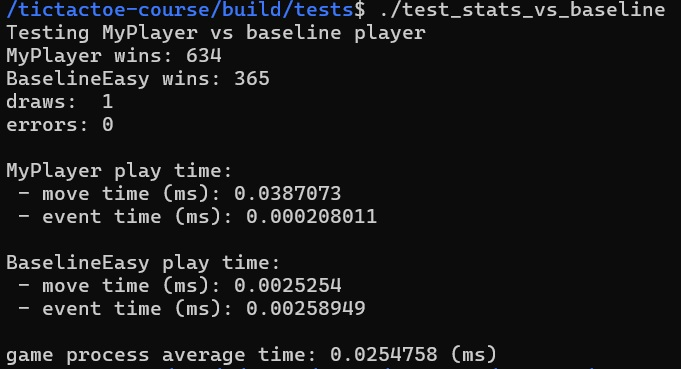
\includegraphics{1}
		\caption{Результат серии игр MyPlayer/BaselineEasy Player}
		
		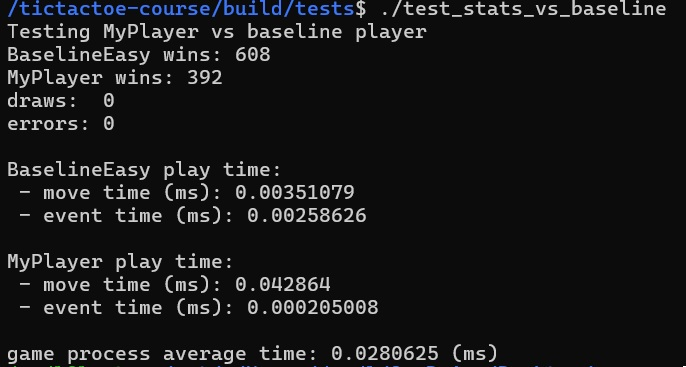
\includegraphics{2}
		\caption{Результат серии игр BaselineEasy Player/MyPlayer}
	\end{figure}
	
	Время расчета хода:
	
	\begin{itemize}
		\item Среднее время хода MyPlayer: 0.0258 мс
		\item Среднее время хода BaselineEasy: 0.0030 мс
		\item Среднее время обработки игры: 0.0268 мс
	\end{itemize}
	
	В первой серии тестовых игр алгоритм одержал 634 победы против 365 поражений при одной ничьей. Это соответствует 63.4\% побед, что превышает целевой показатель в 50\%. Отсутствие ошибок (0 errors) подтверждает надежность реализации алгоритма.
	
	Во второй серии алгоритм одержал 392 победы против 608 поражений без ничьих (39.2\% побед). Ошибки полностью отсутствуют. Данные результаты неудовлетворительны, т. к. требование в виде 50\% побед не пройдено. Для улучшения результатов требуется доработка алгоритма и изменение кода бота.
	
	\item Тестирование против самого себя
	
	Для проверки сбалансированности алгоритма была проведена серия из 1000 игр. На рис. 3 представлены результаты тестов.
	
	\begin{figure}[H]
		\centering
		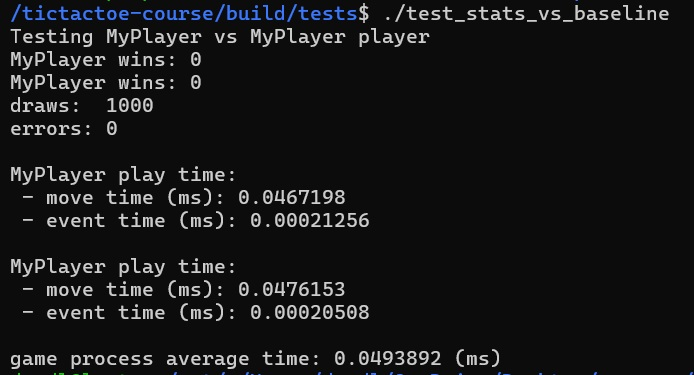
\includegraphics{3}
		\caption{Результат серии игр MyPlayer/MyPlayer}
	\end{figure}
	
	\begin{itemize}
		\item Среднее время хода первого MyPlayer: 0.0467 мс
		\item Среднее время хода второго MyPlayer: 0.0476 мс
		\item Среднее время обработки игры: 0.0494 мс
	\end{itemize}
	
	При игре против самого себя алгоритм демонстрирует идеальную сбалансированность. Время расчета хода менее 50 мс, что соответствует требованию ко времени хода.
\end{enumerate}
\clearpage

\section*{Заключение}
\addcontentsline{toc}{section}{Заключение}

В ходе выполнения курсовой работы была успешно решена поставленная задача разработки алгоритма для игры в крестики-нолики на поле увеличенного размера. 

Разработан и реализован алгоритм, основанный на системе приоритетных правил, который демонстрирует стабильную работу и конкурентоспособность против базового игрока. Написан код класса `MyPlayer` объемом 310 строк на C++, который корректно интегрирован в предоставленную кодобазу и реализует интерфейс `IPlayer`.

Общее время разработки алгоритма и кода: 40 часов. Объем кода: 310 строк реализации и 35 строк заголовочного файла. Общее время написания отчета: 5 часов.

Основным слабым местом реализации является нестабильность результатов - разброс между лучшей (63,4\%) и худшей (39,2\%) сериями составляет 24,2\%. Это свидетельствует о недостаточной адаптивности алгоритма к различным игровым ситуациям.

Для улучшения результатов можно реализовать механизм предсказания ходов противника на 2-3 шага вперед. Также для улучшения результатов можно разработать систему весовых коэффициентов для оценки позиций.
\clearpage

\section*{Список литературы}
\addcontentsline{toc}{section}{Список литературы}

\begin{enumerate}
	\item Полубенцева М. И. C/C++. Процедурное программирование. Санкт-Петербург: БХВ-Петербург, 2008. — 448 с.
	\item Т. А. Павловская. C/C++ Программирование на языке высокого уровня. Санкт-Петербург: Питер, 2003. — 461 с.
	\item Т. А. Павловская, Ю. А. Щупак. C++. Объектно-ориентированное программирование. Практикум. СПб: Питер, 2005. — 265 с.
\end{enumerate}

\clearpage

\renewcommand{\thesection}{\Alph{section}}
\setcounter{section}{0}
\section*{Приложение}
\addcontentsline{toc}{section}{Приложение}

\section{my\_player.cpp}

\begin{lstlisting}[language=C++]
	#include "my_player.hpp"
	#include <cstdlib>
	#include <cstring>
	
	namespace ttt::my_player {
		
		MyPlayer::~MyPlayer( void )
		{
			if (m_board != nullptr)
			{
				for (int i = 0; i < m_rows; i++)
				delete[] m_board[i];
				delete[] m_board;
			}
		}
		
		void MyPlayer::set_sign( Sign sign )
		{ 
			m_sign = sign; 
		}
		
		const char *MyPlayer::get_name( void ) const
		{ 
			return m_name; 
		}
		
		void MyPlayer::initialize_board( const State &state)
		{
			if (m_board != nullptr) 
			return;
			
			m_cols = state.get_opts().cols;
			m_rows = state.get_opts().rows;
			
			m_board = new Sign*[m_rows];
			
			for (int i = 0; i < m_rows; i++)
			{
				m_board[i] = new Sign[m_cols];
				
				for (int j = 0; j < m_cols; j++)
				m_board[i][j] = Sign::NONE;
			}
		}
		
		void MyPlayer::update_board( const State &state)
		{
			initialize_board(state);
			
			for (int y = 0; y < m_rows; y++) 
			{
				for (int x = 0; x < m_cols; x++)
				{
					Sign current_state = state.get_value(x, y);
					
					if (m_board[y][x] != current_state)
					m_board[y][x] = current_state;
				}
			}
		}
		
		int MyPlayer::check_line( int x, int y, int dx, int dy, Sign sign ) const
		{
			int count = 0;
			int max_count = 0;
			
			for (int dir = -1; dir <= 1; dir += 2)
			{
				count = 0;
				
				for (int i = 1; i <= 4; i++)
				{
					int nx = x + i * dx * dir;
					int ny = y + i * dy * dir;
					
					if (nx < 0 || nx >= m_cols || ny < 0 || ny >= m_rows)
					break;
					if (m_board[ny][nx] == sign)
					count++;
					else if (m_board[ny][nx] == Sign::NONE)
					break;
					else
					{
						count = 0;
						break;
					}
				}
				max_count += count;
			}
			
			return max_count;
		}
		
		bool MyPlayer::find_win_move( Point &result, Sign sign ) const
		{
			for (int y = 0; y < m_rows; y++)
			{
				for (int x = 0; x < m_cols; x++)
				{
					if (m_board[y][x] != Sign::NONE)
					continue;
					
					int directions[4][2] = {{1, 0}, {0, 1}, {1, 1}, {1, -1}};
					
					for (int d = 0; d < 4; d++)
					{
						int dx = directions[d][0];
						int dy = directions[d][1];
						
						if (check_line(x, y, dx, dy, sign) >= 4)
						{
							result.x = x;
							result.y = y;
							return true;
						}
					}
				}
			}
			return false;
		}
		
		bool MyPlayer::find_block_move( Point &result, Sign enemy_sign, int threat_level ) const
		{
			for (int y = 0; y < m_rows; y++)
			{
				for (int x = 0; x < m_cols; x++)
				{
					if (m_board[y][x] != Sign::NONE)
					continue;
					
					int directions[4][2] = {{1, 0}, {0, 1}, {1, 1}, {1, -1}};
					
					for (int d = 0; d < 4; d++)
					{
						int dx = directions[d][0];
						int dy = directions[d][1];
						
						int threat = check_line(x, y, dx, dy, enemy_sign);
						
						if (threat >= threat_level)
						{
							result.x = x;
							result.y = y;
							return true;
						}
					}
				}
			}
			return false;
		}
		
		bool MyPlayer::find_double_threat( Point &result, Sign sign ) const
		{
			for (int y = 0; y < m_rows; y++)
			{
				for (int x = 0; x < m_cols; x++)
				{
					if (m_board[y][x] != Sign::NONE)
					continue;
					
					int threat_count = 0;
					int directions[4][2] = {{1, 0}, {0, 1}, {1, 1}, {1, -1}};
					
					for (int d = 0; d < 4; d++)
					{
						int dx = directions[d][0];
						int dy = directions[d][1];
						
						if (check_line(x, y, dx, dy, sign) >= 2)
						{
							threat_count++;
							
							if (threat_count >= 2)
							{
								result.x = x;
								result.y = y;
								return true;
							}
						}
					}
				}
			}
			return false;
		}
		
		bool MyPlayer::find_strategic_move( Point &result, Sign sign ) const
		{
			int center_x = m_cols / 2;
			int center_y = m_rows / 2;
			
			for (int radius = 0; radius <= center_x; radius++)
			{
				for (int y = center_y - radius; y <= center_y + radius; y++)
				{
					for (int x = center_x - radius; x <= center_x + radius; x++)
					{
						if (x < 0 || x >= m_cols || y < 0 || y >= m_rows)
						continue;
						if (m_board[y][x] == Sign::NONE)
						{
							for (int dy = -1; dy <= 1; dy++)
							{
								for (int dx = -1; dx <= 1; dx++)
								{
									if (dx == 0 && dy == 0)
									continue;
									
									int nx = x + dx;
									int ny = y + dy;
									
									if (nx < 0 || nx >= m_cols || ny < 0 || ny >= m_rows)
									continue;
									if (m_board[ny][nx] != Sign::NONE)
									{
										result.x = x;
										result.y = y;
										return true;
									}
								}
							}
						}
					}
				}
			}
			return false;
		}
		
		bool MyPlayer::find_any_move( Point &result) const
		{
			for (int y = 0; y < m_rows; y++)
			{
				for (int x = 0; x < m_cols; x++)
				{
					if (m_board[y][x] == Sign::NONE)
					{
						result.x = x;
						result.y = y;
						return true;
					}
				}
			}
			return false;
		}
		
		Point MyPlayer::make_move( const State &state )
		{
			Point result;
			
			if (state.get_move_no() == 0)
			{
				result.x = state.get_opts().cols / 2;
				result.y = state.get_opts().rows / 2;
				return result;
			}
			
			update_board(state);
			
			Sign enemy_sign = (m_sign == Sign::X) ? Sign::O : Sign::X;
			
			if (find_win_move(result, m_sign)) return result;           
			if (find_block_move(result, enemy_sign, 4)) return result;  
			if (find_double_threat(result, m_sign)) return result;      
			if (find_block_move(result, enemy_sign, 3)) return result;  
			if (find_strategic_move(result, m_sign)) return result;     
			
			for (int attempt = 0; attempt < 50; attempt++)
			{
				result.x = std::rand() % m_cols;
				result.y = std::rand() % m_rows;
				
				if (m_board[result.y][result.x] == Sign::NONE)
				{
					for (int dy = -1; dy <= 1; dy++)
					{
						for (int dx = -1; dx <= 1; dx++)
						{
							if (dx == 0 && dy == 0)
							continue;
							int nx = result.x + dx;
							int ny = result.y + dy;
							if (nx >= 0 && nx < m_cols && ny >= 0 && ny < m_rows && m_board[ny][nx] != Sign::NONE)
							return result;
						}
					}
				}
			}
			
			if (find_any_move(result))
			return result;
			
			result.x = 0;
			result.y = 0;
			return result;
		}
		
	}; // namespace ttt::my_player
\end{lstlisting}
\clearpage

\section{my\_player.hpp}
\begin{lstlisting}[language=C++]
	#pragma once
	
	#include "core/game.hpp"
	
	namespace ttt::my_player {
		
		using game::Event;
		using game::IPlayer;
		using game::Point;
		using game::Sign;
		using game::State;
		
		class MyPlayer : public IPlayer {
			Sign m_sign = Sign::NONE;
			const char *m_name;
			
			Sign** m_board = nullptr;
			int m_cols = 0;
			int m_rows = 0;
			
			public:
			MyPlayer(const char *name) : m_sign(Sign::NONE), m_name(name) {}
			~MyPlayer();
			
			void set_sign(Sign sign) override;
			Point make_move(const State &game) override;
			const char *get_name() const override;
			
			private:
			void initialize_board(const State& state);
			void update_board(const State& state);
			
			int check_line(int x, int y, int dx, int dy, Sign sign) const;
			bool find_win_move(Point& result, Sign sign) const;
			bool find_block_move(Point& result, Sign enemy_sign, int threat_level) const;
			bool find_double_threat(Point& result, Sign sign) const;
			bool find_strategic_move(Point& result, Sign sign) const;
			bool find_any_move(Point& result) const;
		};
		
	}; // namespace ttt::my_player
\end{lstlisting}


\end{document}
